\documentclass[a4paper]{article}
\usepackage[utf8]{inputenc}
\usepackage[russian,english]{babel}
\usepackage[T2A]{fontenc}
\usepackage[left=10mm, top=20mm, right=18mm, bottom=15mm, footskip=10mm]{geometry}
\usepackage{indentfirst}
\usepackage{amsmath,amssymb}
\usepackage{mathastext} 
\usepackage[italicdiff]{physics}
\usepackage{graphicx}
\usepackage{caption}
\usepackage{float}
\usepackage{caption}
\renewcommand{\thefootnote}{\fnsymbol{footnote}}
\usepackage{tablefootnote}
\usepackage{footmisc}
\usepackage{textcomp}
\usepackage{multicol}
\usepackage{multirow}
\usepackage[parfill]{parskip}
\usepackage{makecell}
\usepackage{array}  
\usepackage{siunitx}
\usepackage{booktabs}
\sisetup{
    exponent-product = \cdot,
    per-mode = symbol,
    separate-uncertainty = true,
    uncertainty-separator = \,
}
\renewcommand\cellalign{cc} 
\renewcommand\cellgape{\Gape[2pt]} 
\usepackage[utf8]{inputenc}\newcommand{\approxtext}[1]{\ensuremath{\stackrel{\text{#1}}{\approx}}}
\usepackage[colorlinks=true, urlcolor=blue, linkcolor=blue, citecolor=blue]{hyperref}
\graphicspath{{images/}}
\DeclareGraphicsExtensions{.pdf,.png,.jpg}
\usepackage{wrapfig}
\captionsetup{labelformat=empty}
\usepackage{caption}
\captionsetup[figure]{name=Рисунок}
\captionsetup[table]{name=Таблица}
%\usepackage{newtxtext,newtxmath} 
\title{\textbf{Отчет о выполнении лабораторной работы 3.1.3}}
\date{}
\author{Котляров Михаил, Б01-402}

\begin{document}

\maketitle
	
\section{Введение}

\subsection*{Цель работы}
Исследовать свойства постоянных неодимовых магнитов; измерить с их помощью горизонтальную и вертикальную составляющие индукции магнитного поля Земли и магнитное наклонение.

\subsection*{Оборудование}
Неодимовые магниты; тонкая нить для изготовления крутильного маятника; медная проволока; электронные весы; секундомер; измеритель магнитной индукции; штангенциркуль; брусок, линейка и штатив из немагнитных материалов; набор гирь и разновесов.

\subsection*{Теоретические сведения}
Магнитное поле точечного диполя с магнитным моментом \(\mathbf{m}\) определяется формулой:
\[
\mathbf{B}_{\text{дип}} = \frac{\mu_0}{4\pi} \left( \frac{3(\mathbf{m} \cdot \mathbf{r})\mathbf{r}}{r^5} - \frac{\mathbf{m}}{r^3} \right),
\]
где \(\mu_0 = 4\pi \cdot 10^{-7} \, \text{Гн/м}\).  

Во внешнем магнитном поле с индукцией \(\mathbf{B}\) на диполь действует механический момент сил:
\[
\mathcal{M} = [\mathbf{m} \cdot \mathbf{B}],
\]
а его потенциальная энергия равна:
\[
W = -(\mathbf{m} \cdot \mathbf{B}).
\]

В неоднородном поле на диполь также действует сила:
\[
\mathbf{F} = -\nabla W = (\mathbf{m} \cdot \nabla) \mathbf{B}.
\]

Для однородно намагниченного шара радиусом \(R\) магнитный момент связан с намагниченностью \(M\) соотношением:
\[
\mathbf{m} = M \cdot V, \quad V = \frac{4\pi}{3}R^3.
\]

Остаточная индукция материала определяется как \(B_r = \mu_0 M\), а индукция на полюсах шара вычисляется по формуле:
\[
B_p = \frac{2}{3} B_r.
\]

Магнитное поле Земли характеризуется горизонтальной \(B_{\parallel}\) и вертикальной \(B_{\perp}\) составляющими, а также магнитным наклонением \(\beta\), связанным с ними соотношением:
\[
\tan \beta = \frac{B_{\perp}}{B_{\parallel}}.
\]
\section{Выполнение}

\subsection*{Измерение характеристик магнитных шариков}

\begin{enumerate}
\item Подложим на весы толстую стопку листов, чтобы магнитные шарики не притягивались к металлическим частям весов. Масса листов $m_{\text{листов}} = 145.613$ г, масса 40 шариков на листах $m_{\text{сумм}} = 178.693$ г, масса 1 шарика $m = \frac{m_{\text{сумм}} - m_{\text{листов}}}{40} = 0.827$. Погрешность $\sigma_m = \frac{\sigma_{\text{весов}}}{40} = 0,000025$ г ($\varepsilon_m = 0,003 \%$).
\item Измерим радиус шариков. Длина цепочки из 10 шариков $d_{10} = 5.73$ см, радиус одного шарика $R = 0,2865 \pm 0,0005$ см.

\item Измерим магнитное поле на полюсах шариков.
\begin{table}[h!]
    \centering
    \begin{tabular}{|c|c|}
        \hline
        № & $B_p,\ \text{мТл}$ \\ \hline
        1 & 328 \\ \hline
        2 & 270 \\ \hline
        3 & 238 \\ \hline
        4 & 320 \\ \hline
        5 & 241 \\ \hline
        6 & 230 \\ \hline
        7 & 337 \\ \hline
    \end{tabular}
    \caption{Таблица 1. Измеренные значения индукции магнитного поля на полюсах шариков}
    \label{tab:Bp_measurements}
\end{table}

Рассчитаем среднее: $B_p^{\text{ср}} = 2806 \pm 176$ Гс ($\varepsilon_{B_p^{\text{ср}}} = 6,28 \%$).

\item Магнитный момент шарика $P_m = \frac{B_p^{\text{ср}} R^3}{2} = 32,99 \pm 2,08 \text{ см}^3 \cdot \text{Гс}$ ($\varepsilon_{P_m} = 6,3 \%$), намагниченность $p_m = \frac{P_m}{V} = \frac{P_m}{\frac{4}{3} \pi R^3} = 334,9 \pm 21,2$ Гс, остаточная магнитная индукция $B_r = 4 \pi p_m = 4209 \pm 266$ Гс.

\subsection*{Метод A. Определение магнитного момента по силе отрыва}

    \item Найдём максимальное расстояние $r_{\text{max}}$ между центрами шариков, при котором они ещё удерживают друг друга в поле тяжести:
    \begin{itemize}
        \item Поместим между шариками брусок из немагнитного материала
        \item Будем увеличивать расстояние между шариками.
        \item Измерим расстояние $r_{\text{max}}$ в момент отрыва шариков. 
    \end{itemize}
    
	Получилось $r_{\text{max}} = 2,173 \pm 0,100$ см ($\varepsilon_{r_{\text{max}}} = 4,6 \%$).
    \item Рассчитаем магнитный момент $P_{m}$:
    \[
    P_{m} = \sqrt{\frac{mg r_{\text{max}}^4}{6}} = 54,90 \pm 5,05 \text{ см}^3 \cdot \text{Гс} \ (\varepsilon_{P_m} = 9,2 \%),
    \]
    где $g = 980\ \text{см/с}^2$ -- ускорение свободного падения. Магнитное поле $B_p = \frac{2 P_m}{R^3} = 4669 \pm 430$ Гс ($\varepsilon_{B_p} = 9,22 \%$), намагниченность $p_m = 557,3 \pm 51,4$ Гс, остаточная магнитная индукция $B_r = 4 \pi p_m = 7003 \pm 646$ Гс.

\subsection*{Метод Б. Определение магнитного момента по силе сцепления}

    \item Составим цепочку из 30 магнитных шариков. Будем присоединять к цепочке гири и разновесы, подбирая минимальный вес системы цепочки с гирей, при котором она отрывается от верхнего шарика. Определим с помощью весов массу $m_{\text{ц}}$ оторвавшейся цепочки с гирей. Получилось $m_{\text{ц}} = 353.254$ г, $F = 346424$ дин.
    
    \item Рассчитаем силу сцепления $F_0$ двух шаров по формуле:
    \[
    F_0 = \frac{F}{1,08} = 320761 \text{дин}.
    \]
    Вычислим магнитный момент $P_m$:
    \[
    P_m = R^2 \sqrt{\frac{8F_0}{3}} = 75,91 \pm 2,17 \text{ см}^3 \cdot \text{Гс } (\varepsilon_{P_m} = 2,85 \%), 
    \]
    где $R$ -- радиус шарика. Магнитное поле $B_p = \frac{2 P_m}{R^3} = 6456 \pm 187$ Гс ($\varepsilon_{B_p} = 2,90 \%$), намагниченность $p_m = 770,7 \pm 22,3$ Гс, остаточная магнитная индукция $B_r = 9684 \pm 281$ Гс. \\

Рассчитаем средний магнитный момент по прямому измерению, методу А и Б: $P_m^\text{ср} = \frac{w_\text{прям} P_m^\text{прям} + w_\text{А} P_m^\text{А} + w_\text{Б} P_m^\text{Б}}{w_\text{прям} + w_\text{А} + w_\text{Б}} = 53,68 \pm 2,79\text{ см}^3 \cdot \text{Гс }$

\subsection*{Измерение горизонтальной составляющей магнитного поля Земли}

    \item Соберём крутильный маятник из 12 магнитных шариков и подвесим его на немагнитном штативе с помощью $\Lambda$-образного подвеса. Установим «магнитную стрелку» в горизонтальное положение.
    
    \item Возбудим крутильные колебания маятника вокруг вертикальной оси и измерим их период $T$ с помощью секундомера.
    
    \item Проверим влияние упругости нити на период колебаний:
    \begin{itemize}
        \item Свернём «стрелку» в кольцо (магнитный момент такого маятника равен нулю)
        \item Возбудим крутильные колебания и убедимся, что период существенно не изменяется
    \end{itemize}
    
    \item Исследуем зависимость периода $T$ крутильных колебаний от количества шариков $n$:
    \begin{table}[h!]
    \centering
    \begin{tabular}{|c|c|}
        \hline
        $n$ & $T,\ \text{с}$ \\ \hline
        12 & 3,748 \\ \hline
        10 & 3,158 \\ \hline
        8 & 2,696 \\ \hline
        6 & 1,990 \\ \hline
        4 & 1,350 \\ \hline
        3 & 1,059 \\ \hline
    \end{tabular}
    \caption{Таблица 2. Зависимость периода крутильных колебаний от количества шариков в стрелке}
    \label{tab:T_n}
\end{table}

Построим по МНК график зависимости $T(n)$ и убедимся в его линейности.
    \begin{figure}[h]
        \center{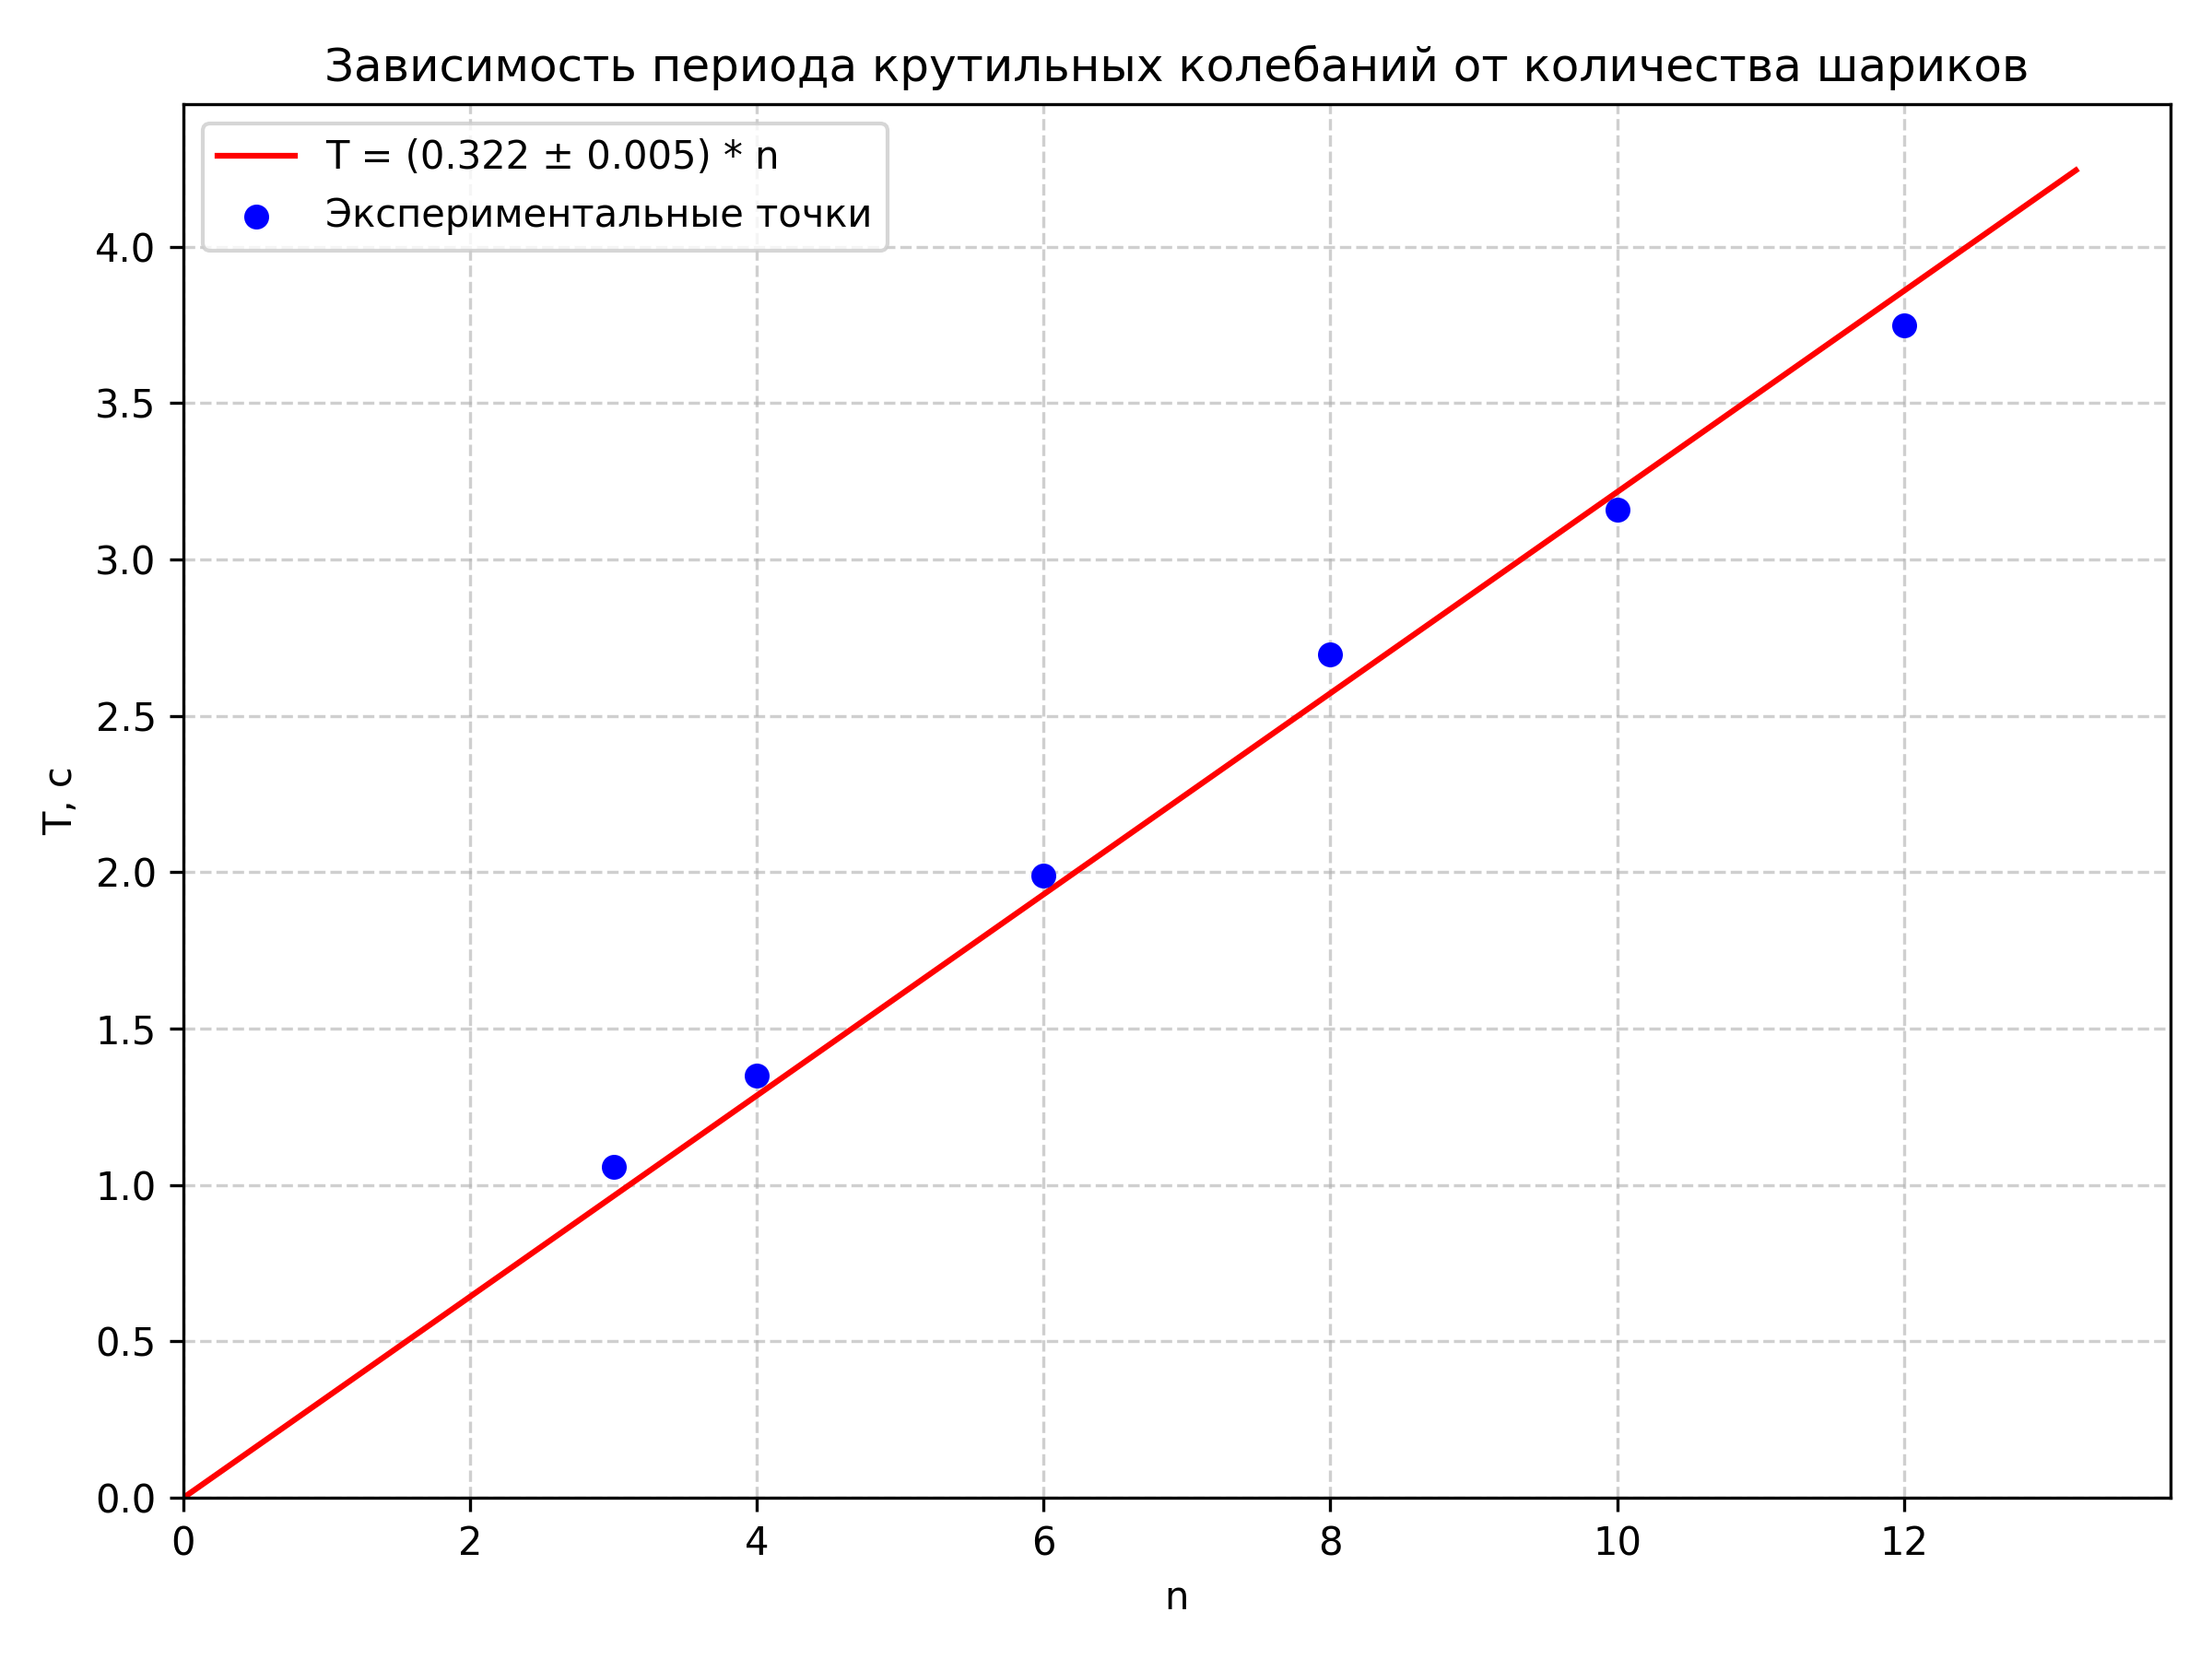
\includegraphics[width=0.7\textwidth]{Graphics/T_vs_n.png}}
        \caption{График 1. Зависимость периода крутильных колебаний от числа шариков}
\end{figure}
\\Наклон прямой $k = 0,322 \pm 0,005$ с ($\varepsilon_k = 1,55 \%$).
    \item Рассчитаем горизонтальную составляющую $B_{\parallel}$ по угловому коэффициенту графика:
    \[
    B_{\parallel} = \frac{4\pi^2 m R^2}{3P_m k^2} = 0,160 \pm 0,010 \text{ Гс} (\varepsilon_{B_{\parallel}} = 6,06 \%),
    \]
    где $k$ -- угловой коэффициент зависимости $T(n)$, $P_m$ - средний магнитный момент шариков, рассчитанный как взвешенное среднее по методам А и Б.

\subsection*{III. Измерение вертикальной составляющей и магнитного наклонения}

    \item Изготовим магнитную «стрелку» из $n = 10$ шариков и подвесим её за середину на нити.
    
    \item Определим механический момент сил, действующий на «стрелку»:
    \begin{itemize}
        \item С помощью кусочков медной проволоки уравновесим «стрелку» в горизонтальном положении
        \item Измерим массу уравновешивающего груза $m_{\text{гр}}$ на весах
    \end{itemize}
    
    \item Рассчитаем механический момент сил:
    \[
    \mathcal{M} = m_{\text{гр}} g r_{\text{гр}},
    \]
    где $r_{\text{гр}}$ -- плечо силы тяжести.
    
\begin{table}[h!]
    \centering
    \begin{tabular}{|c|c|c|c|}
        \hline
        $n$ & $\text{плечо},\ \text{см}$ & $m_{\text{гр}},\ \text{г}$ & $\mathcal{M},\ \text{дин}\cdot\text{см}$ \\ \hline
        12 & 2,292 & 0,127 & 285,46 \\ \hline
        10 & 2,292 & 0,101 & 227,02 \\ \hline
        8 & 1,719 & 0,127 & 214,09 \\ \hline
        6 & 1,146 & 0,170 & 191,05 \\ \hline
        4 & 0,573 & 0,319 & 179,25 \\ \hline
    \end{tabular}
    \caption{Таблица 3. Зависимость механического момента сил от количества шариков в стрелке}
    \label{tab:M_n}
\end{table}
    
    \item Построим график зависимости $\mathcal{M}(n)$ и убедимся в его линейности.
        \begin{figure}[h]
        \center{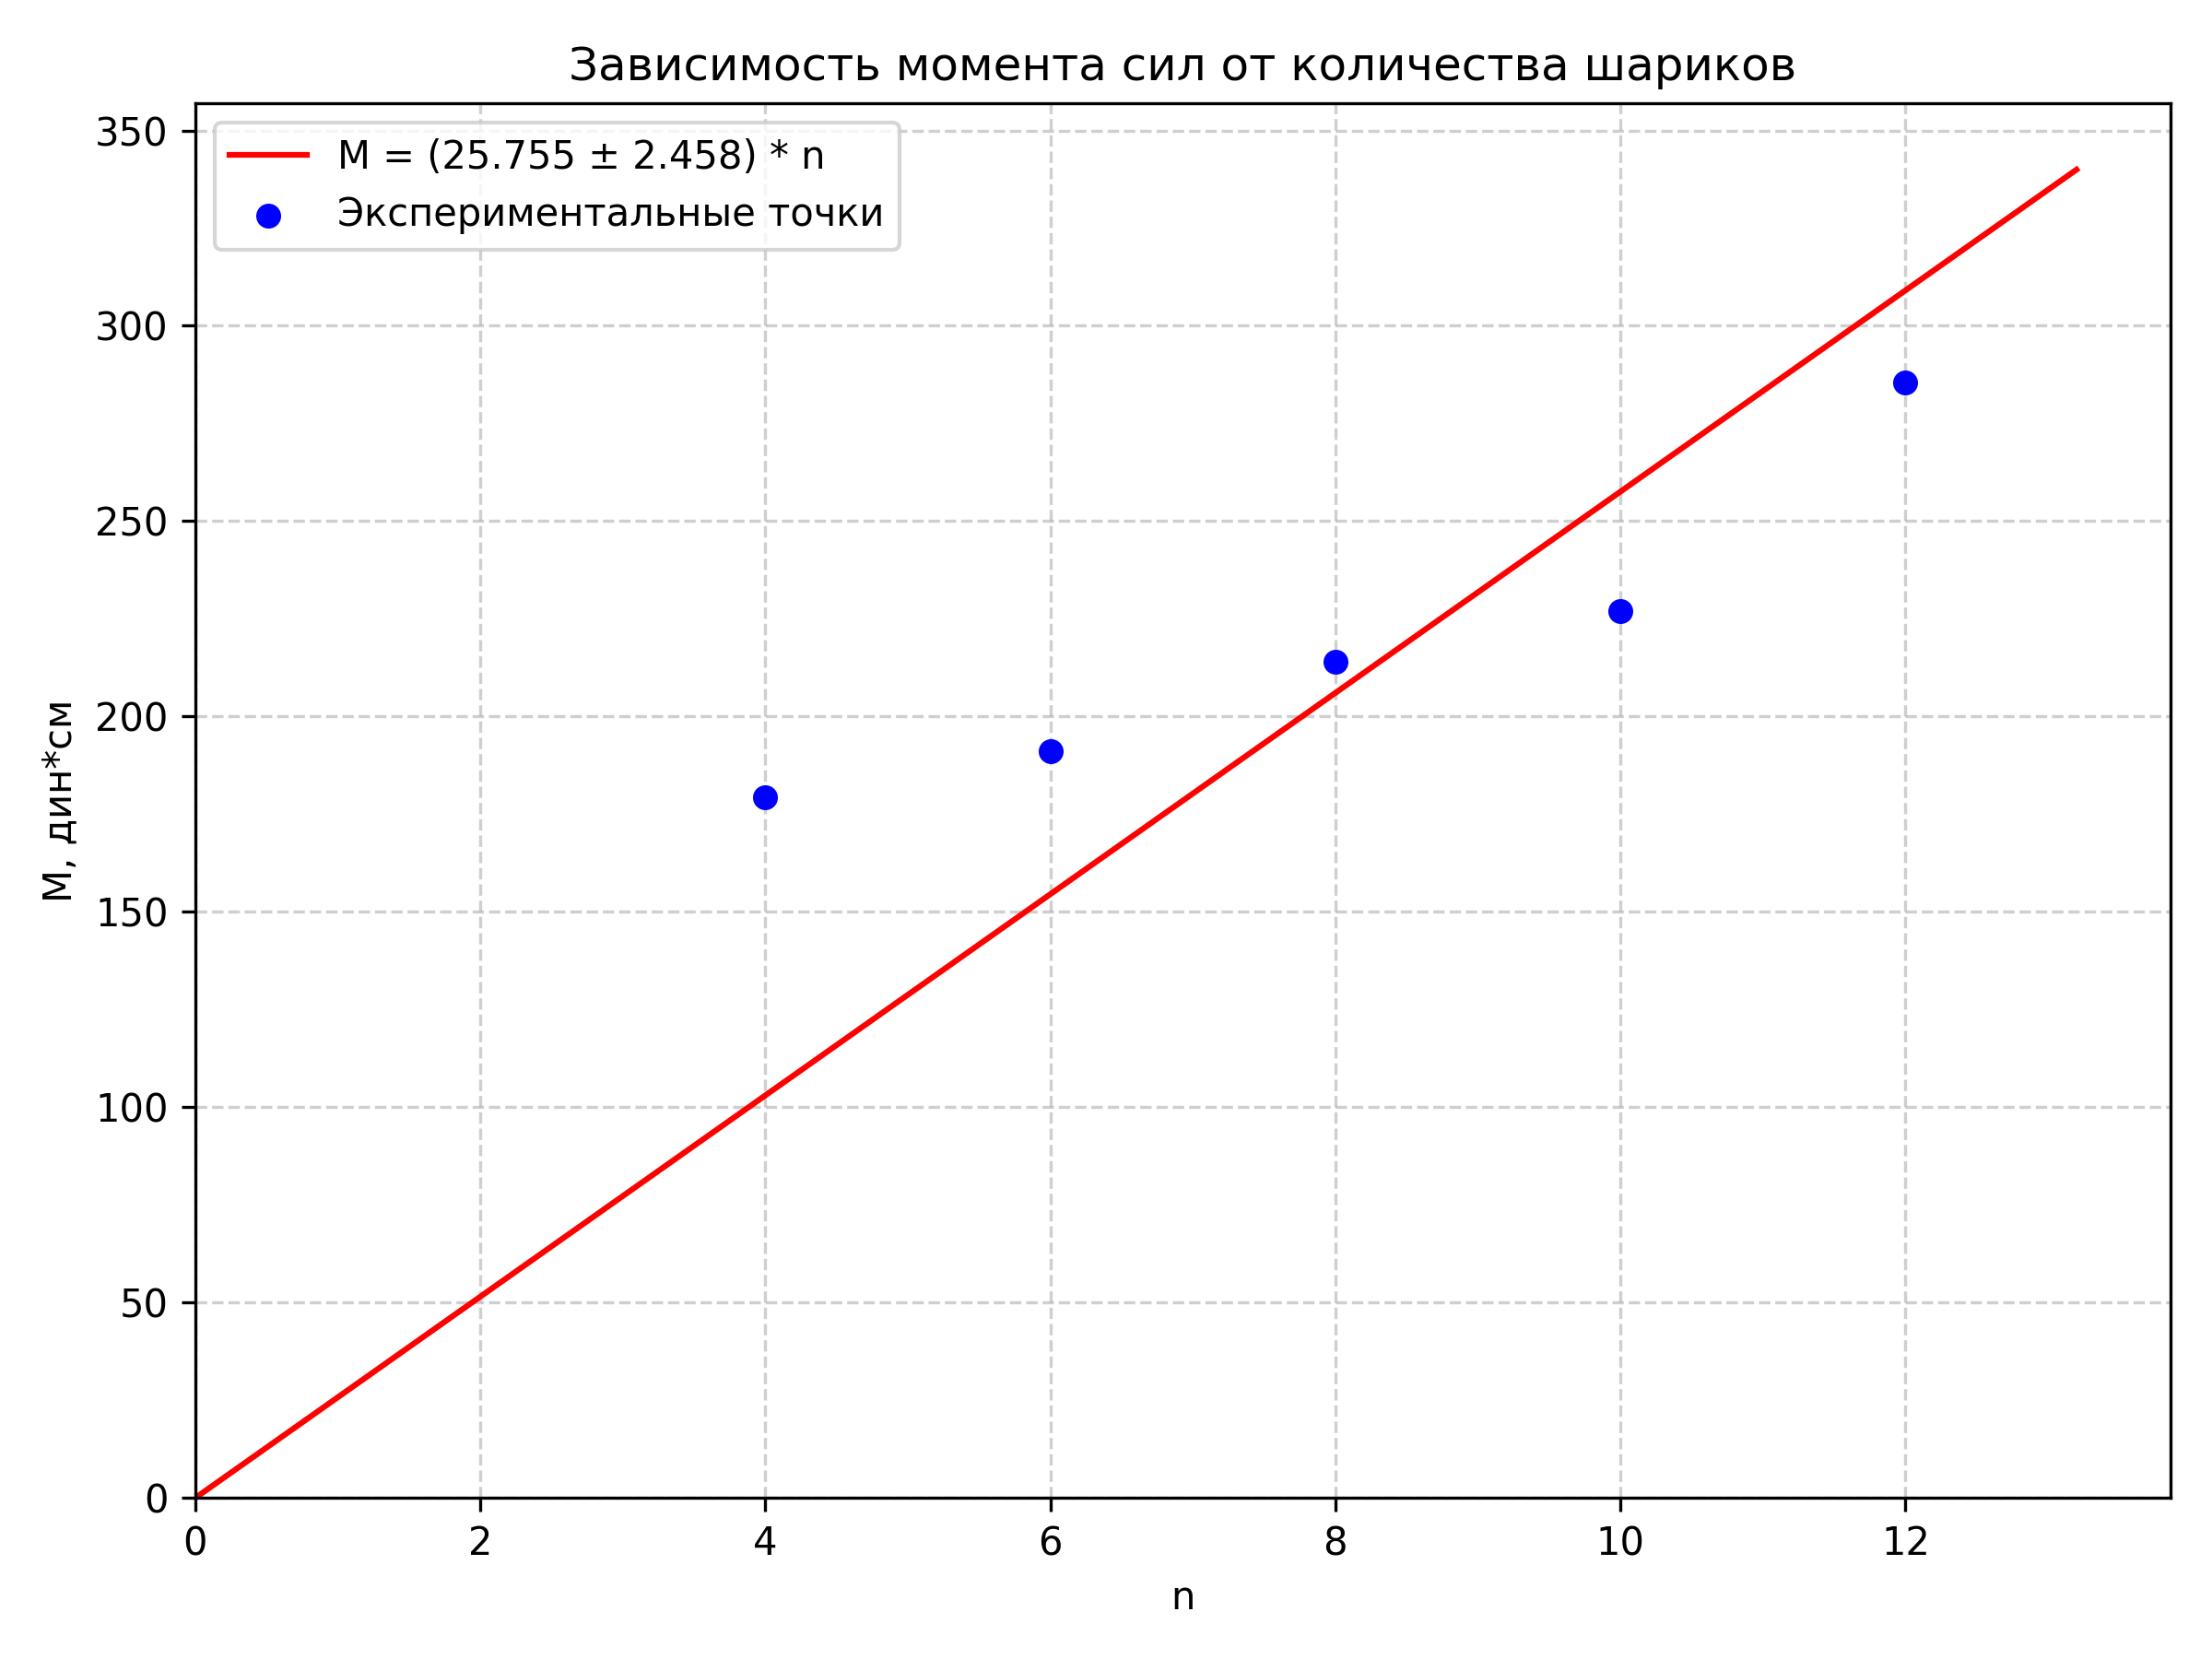
\includegraphics[width=0.7\textwidth]{Graphics/M_vs_n.png}}
        \caption{График 2. Зависимость момента сил от количества шариков}
\end{figure}
\\Наклон прямой $k_{\mathcal{M}} = 25,76 \pm 2,46$ дин$\cdot$см ($\varepsilon_k = 9,54\%$).
    \item Рассчитаем вертикальную составляющую $B_{\perp}$ по угловому коэффициенту графика:
    \[
    B_{\perp} = \frac{k_{\mathcal{M}}}{P_m} = 0,480 \pm 0,052 \text{ Гс } (\varepsilon_{B_{\perp}} = 10,86 \%),
    \]
    где $k_{\mathcal{M}}$ -- угловой коэффициент зависимости $\mathcal{M}(n)$.

\subsection*{Рассчет характеристик магнитного поля Земли}   
    \item Определим магнитное наклонение $\beta$:
    \[
    \tan \beta = \frac{B_{\perp}}{B_{\parallel}} = 1,248 \pm 0,037 \text{ рад} = 71,50^\circ \pm 2,14^\circ \ (\varepsilon_{\beta} = 3,00 \%).
    \]
    
    \item Найдём полную величину индукции магнитного поля Земли:
    \[
    B_{\text{Земли}} = \sqrt{B_{\parallel}^2 + B_{\perp}^2} = 0,506 \pm 0,050 \text{ Гс } (\varepsilon_{B_{\text{Земли}}} = 9,79\%).
    \]
    
	\item Рассчитаем магнитный момент Земли:

Исходные данные
\begin{itemize}
    \item Географическая широта: $\varphi \approx 56^\circ$ N
    \item Горизонтальная компонента: $B_{\parallel} = 0,160 \pm 0,010 \text{ Гс}$
    \item Угол наклонения: $\beta = 71,50^\circ \pm 2,14^\circ$
    \item Радиус Земли: $R = 6.371 \cdot 10^8\,\text{см}$
\end{itemize}

Расчёт:\\
\textbf{Магнитная широта:}
        \[
        \theta = \arctan \left( \frac{1}{2} \tan \beta \right) = 0,981 \pm 0,057 \text{ рад } (\varepsilon_{\theta} = 5,86 \%)
        \]
    
\textbf{Поле на экваторе:}
        \[
        B_{\text{экв}} = \frac{B_h}{\cos \theta} = 0,289\pm 0,030 \text{ Гс } (\varepsilon_{B_{\text{экв}}} = 10,52\%)
        \]
    
\textbf{Магнитный момент:}
        \[
        P_m^\text{Земли} = B_{\text{экв}} \cdot R^3 = 0,289 \cdot (6.371 \cdot 10^8)^3 = (7,46 \pm 0,78) \cdot 10^{25} \text{ см}^3 \cdot \text{Гс}
        \]

\end{enumerate}


\section{Результаты и обсуждения}

\begin{enumerate}
\item Сравним три метода измерения магнитных характеристик шариков и табличное значение остаточной индукции:

\begin{table}[h!]
    \centering
    \begin{tabular}{|c|c|c|c|c|}
        \hline
        Метод & $P_m$, см$^3\cdot$Гс & $B_p$, Гс & $p_m$, Гс & $B_r$, Гс \\ \hline
        Прямое измерение & $32,99 \pm 2,08$ & $2806 \pm 176$ & $334,9 \pm 21,2$ & $4209 \pm 266$ \\ \hline
        Метод А & $54,90 \pm 5,05$ & $4669 \pm 430$ & $557,3 \pm 51,4$ & $7003 \pm 646$ \\ \hline
        Метод Б & $75,91 \pm 2,17$ & $6456 \pm 187$ & $770,7 \pm 22,3$ & $9684 \pm 281$ \\ \hline
    \end{tabular}
    \caption{Таблица 4. Сравнение методов определения магнитных параметров}
    \label{tab:methods_comparison}
\end{table}

Табличная остаточная индукция Неодим-железо-бор $Nd_2Fe_{14}B$ $B_r^\text{табл}\footnotemark[1] = 12200$ Гс. Ближе всего к табличному значению оказался метод Б, прямое измерение показало наихудший результат.
\footnotetext[1]{Табличное значение остаточная индукция Неодим-железо-бор $Nd_2Fe_{14}B$ взято из книги Лабораторный практикум по общей физике Том 2 Электричество и магнетизм под ред. Максимычева}

\item Сравним магнитные характеристики Земли, полученные в ходе эксперимента, с табличными:
\begin{table}[h!]
    \centering
    \begin{tabular}{|c|c|c|c|c|c|}
        \hline
        & $B_{\parallel}$, Гс & $B_{\perp}$, Гс & $B$, Гс & $\beta$, $^\circ$ & $P_m^\text{Земли}, \text{ см}^3 \cdot \text{Гс}$ \\ \hline
        Экспериментальные & $0,160 \pm 0,010$ & $0,480 \pm 0,052$ & $0,506 \pm 0,050$ & $71,50 \pm 2,14$ & $(7,46 \pm 0,785) \cdot 10^{25}$ \\ \hline
        Табличные\footnotemark[2] & $0,165599$ & $0,504311$ & $0,530804$ & $71,8216$ & $7,7 \cdot 10^{25}$ \\ \hline
    \end{tabular}
    \caption{Таблица 5. Сравнение экспериментальных и табличных значений параметров магнитного поля Земли}
    \label{tab:earth_field_comparison}
\end{table}
\end{enumerate}

Как мы видим, все значения сходятся с высокой точностью.
\footnotetext[2]{Табличные значения взяты с сайта \url{https://www.ngdc.noaa.gov/geomag/calculators/magcalc.shtml\#igrfwmm}, координаты брались: 55.929444 N, 37.518434 E, время обращения 31.10.2025}
\section{Вывод}

В ходе лабораторной работы были исследованы свойства неодимовых магнитов и измерены параметры магнитного поля Земли. 

Были определены магнитные характеристики шариков тремя методами. Наилучшее согласование с табличными значениями для NdFeB показал метод Б тогда как методы А и прямого измерения дали заниженные результаты, что может быть связано с приближённым характером используемых формул и трудностью точного определения точки отрыва.

Экспериментально измерены составляющие магнитного поля Земли: горизонтальная $B_{\parallel} = 0,160 \pm 0,010$ Гс и вертикальная $B_{\perp} = 0,480 \pm 0,052$ Гс. Полученное магнитное наклонение $\beta = 71,50^\circ \pm 2,14^\circ$ и полная индукция $B = 0,506 \pm 0,050$ Гс хорошо согласуются с табличными значениями для Долгопрудного.

Подтверждена линейная зависимость периода крутильных колебаний и механического момента от количества шариков в стрелке, что свидетельствует о аддитивности магнитных моментов и магнитожёсткости материала неодимовых магнитов.
\end{document}